% SafeDecontam -- canonical five-page camera-ready source.
% Approved scientific text and citation order are frozen; no alternate prose branches.
\documentclass[conference]{IEEEtran}
\IEEEoverridecommandlockouts
\usepackage{cite}
\usepackage{amsmath,amssymb,amsfonts}
\usepackage{graphicx}
\usepackage{booktabs}
\usepackage{textcomp}
\usepackage{xcolor}
\usepackage[T1]{fontenc}
\usepackage[utf8]{inputenc}
\usepackage{microtype}
\usepackage{url}
% The approved compact title spacing is retained to meet the five-page limit.
% This is a documented title-spacing exception to the unmodified template.
% Margins, column widths, body font size and body baselines are unchanged.
\makeatletter
\def\@IEEEauthorblockconfadjspace{-18pt}
\let\orig@maketitle\@maketitle
\def\@maketitle{\orig@maketitle\vspace{-30pt}}
\makeatother
\def\BibTeX{{\rm B\kern-.05em{\sc i\kern-.025em b}\kern-.08em T\kern-.1667em\lower.7ex\hbox{E}\kern-.125emX}}

% Stable PDF metadata for repeat builds in the same TeX toolchain.
\pdfinfoomitdate=1
\pdftrailerid{}
\pdfsuppressptexinfo=15
\begin{document}

\title{SafeDecontam: Risk-Controlled Benchmark\\Decontamination}

\author{
\IEEEauthorblockN{Chuhong Xu\IEEEauthorrefmark{1}}
\thanks{\IEEEauthorrefmark{1}Corresponding author: Chuhong Xu (chuhong.xu@sony.com).}
\IEEEauthorblockA{\textit{Sony Corporate of America}\\San Jose, USA\\chuhong.xu@sony.com}
\and
\IEEEauthorblockN{Hang Xiao}
\IEEEauthorblockA{\textit{Fortinet, Inc.}\\Sunnyvale, USA\\xhang@fortinet.com}
\and
\IEEEauthorblockN{Zhaoyi Li}
\IEEEauthorblockA{\textit{Intuit Inc.}\\Mountain View, USA\\lzy9776@gmail.com}
}

\maketitle

\begin{abstract}
Benchmark corpus filtering requires an explicit operating point: permissive rules leave leakage in place, whereas aggressive rules delete legitimate related material. SafeDecontam is a source-level deletion rule applied after an upstream retriever returns candidate documents for known benchmark items. Its evidence adapter combines lexical similarity, constraint agreement, answer support, chronology, and page-level pooling; the scorer is fixed before calibration. For each source item, calibration applies an exact one-sided tolerance procedure to the largest score among retain-labeled candidates, and the method abstains when the clean calibration reservoir cannot support the requested collateral-deletion budget. We evaluate SafeDecontam on constructed pairs from public benchmark artifacts and on raw web-search evidence; in a blinded and adjudicated Massive Multitask Language Understanding (MMLU) audit, it achieves 81.71 percent recall, 100 percent precision, and 0.9894 area under the receiver operating characteristic curve (AUROC), with no clean removals among 71 items (one-sided 95 percent exact upper bound 4.13 percent). Recall drops on external benchmark families and a cross-lingual probe, so evidence coverage and calibration data must be established for each family. SafeDecontam is thus a corpus-deletion policy for retrieved candidates with an explicit damage budget and abstention condition; it does not establish model training exposure or score inflation.
\end{abstract}

% Exactly one author-requested blank abstract line.
\vspace{10pt}
\begin{IEEEkeywords}
benchmark contamination, corpus filtering, risk control, data governance, large language models
\end{IEEEkeywords}

\section{Introduction}
Open benchmarks support reproducible model comparisons, but the same accessibility exposes questions, worked solutions, and minor variants to data-collection pipelines~\cite{sainz2023}, and evaluation scores may then mix generalization with prior exposure even when a prompt does not reproduce stored text verbatim~\cite{deng2024}. Contamination studies usually begin after training: protected or transformed evaluations test robustness to a changed surface~\cite{jacovi2023}, and retrieval audits locate likely source matches~\cite{li2024}. Corpus curation instead asks what can be removed before training and at what cost. Literal overlap is a poor boundary here: rephrasing or translation may preserve decisive content while changing nearly every local string~\cite{yang2023}, while tutorials, earlier sources, and same-topic questions share vocabulary without revealing the answer.

The central problem is threshold selection under asymmetric error costs: a permissive cutoff misses derivatives, an aggressive cutoff removes more legitimate material, and pairwise AUROC ranks candidate records but neither specifies a tolerable deletion risk nor reveals how false removals spread across benchmark source items during corpus-wide screening.

SafeDecontam formulates the decision over source groups: a replaceable scorer maps the adapter's evidence to a removal score, the largest retain score in each group calibrates a one-sided non-parametric tolerance threshold once validation fixes the scorer, and a cutoff is returned only when clean groups support the requested budget.

Experiments cover a constructed pool from three public benchmark ecosystems and released MMLU search results, with source groups kept intact across partitions. This paper contributes (i)~a source-level definition of collateral deletion, where a source is damaged if any legitimate related candidate is removed; (ii)~an auditable evidence adapter and an exact clean-only calibration rule that meets a pre-specified damage budget or abstains; and (iii)~a group-preserving evaluation with a separated raw-search protocol whose final MMLU decisions are checked by blinded human adjudication.

\subsection{Scope and Threat Model}
SafeDecontam operates after an upstream retriever has produced candidate documents for a known benchmark item, and considers accidental or non-adaptive benchmark reuse, including exact copies, paraphrases, translations, and answer-bearing fragments. It neither guarantees recall for candidates missed by retrieval nor defends against an adaptive adversary optimizing content against the frozen adapter or threshold. The protected asset is legitimate corpus material; the controlled loss is the probability that at least one retain-labeled candidate of a source item is deleted. The guarantee assumes a fixed scorer, evidence schema, and labeling rule, with clean groups drawn from the same within-family distribution as the calibration reservoir; label noise, a change of benchmark family, language, or retrieval source, or a changed parser or encoder voids it, and Section~\ref{sec:reservoir} states how a reservoir is built for each family.

\section{Related Work}
Contamination audits operate on two surfaces: corpus-side methods search for source material, whereas model-side probes measure behavior consistent with prior exposure. Shingle containment offers an inexpensive exact-match baseline~\cite{broder1997}, and Okapi Best Matching 25 (BM25) adds term weighting and query normalization~\cite{robertson2009}. Both remain lexical: neither encodes answer preservation, chronology, or structured numerical changes, and their evidence weakens as a derivative moves away from literal reuse.

Risk-controlling prediction sets supply the statistical template~\cite{bates2021}: grouping retain candidates by source and calibrating their maximum score aligns the calibration variable with the deletion event of interest, and a one-sided tolerance limit on these maxima controls source-group damage directly.



\section{Method}
\subsection{Decision Unit and Losses}
For benchmark item $b$ and candidate document $d$, let $s(b,d)$ denote an increasing removal score. All candidates associated with $b$ form source group $g$; grouping makes the deletion event explicit, since damage occurs when the policy removes any legitimate material linked to the same benchmark item.

\begin{table}[t]
\caption{Constructed Pair Pool by Family.\\GSM8K: Grade School Math 8K; MCQ: Multiple Choice.}
\label{tab:pool}
\centering
\begin{tabular}{lrrr}
\toprule
Family & Groups & Remove & Retain\\
\midrule
Arithmetic (GSM8K) & 1,319 & 5,272 & 6,873\\
MCQ (MMLU) & 505 & 2,000 & 1,515\\
MATH Level 5 & 253 & 506 & 1,012\\
\midrule
Total & 2,077 & 7,778 & 9,400\\
\bottomrule
\end{tabular}
\end{table}

The remove class contains exact copies, verified derivatives such as released rephrasings~\cite{yang2023} and answer-preserving mathematical variants~\cite{li2024gsmplus}, and answer-bearing fragments. The retain class includes changed-answer perturbations even when they remain close to the source on the surface~\cite{mirzadeh2024}, together with same-topic items, predating sources, and unrelated controls.

At threshold $\tau$, pair contamination recall (CR) and pair collateral deletion rate (CDR) are
\begin{equation}
\mathrm{CR}=\Pr[s\ge\tau\mid Y=1],\qquad \mathrm{CDR}=\Pr[s\ge\tau\mid Y=0].
\label{eq:pair}
\end{equation}
A source item incurs damage when any of its legitimate candidates is deleted; group collateral deletion rate (GCDR) measures the fraction of source groups with at least one removed retain candidate. CR and CDR summarize pairwise behavior; GCDR captures whether a small pairwise error is dispersed across many benchmark items at deployment scale. In the constructed pool, CR and CDR are pair-level and GCDR is group-level; in the raw-search audit, each source item forms one group after page-level pooling, so reported recall and clean-removal rates are source-item quantities, not the pair-level rates in~(\ref{eq:pair}).

\subsection{Observable Evidence and Score Models}
Six similarity features form the lexical layer. Four-gram containment and three-shingle Jaccard measure local reuse~\cite{broder1997}; query-normalized BM25 supplies term-weighted retrieval~\cite{robertson2009}. Word- and character-level term frequency--inverse document frequency (TF--IDF) cosines capture broader overlap, while a 64-dimensional latent-semantic cosine provides a low-rank view; vocabulary construction and projection fitting are confined to the training partition.

Structured MATH perturbations show why lexical similarity cannot determine whether a changed number reverses the answer~\cite{huang2025}. The adapter records numbers, relation cues, target tokens, entities, and units; counts answer support only in conclusion-like context; checks the first four available constraints; and uses chronology only with a reliable predating source~\cite{miao2020}.

Candidate scorers include each individual feature, their mean, no-constraint (similarity-plus-chronology) and full-evidence logistic models, and a 16-unit multilayer perceptron (MLP) with rectified-linear-unit activation, quasi-Newton optimization, and $\ell_2$ regularization; validation selects one scorer before calibration begins. MLP thresholds use the unsquashed margin, which avoids boundary ties from saturated logits. The protocol separates fitting, calibration on clean-group maxima, and one-time evaluation under the locked decision rule.

\subsection{Clean-Only Exact Calibration}
For family $h$, let $R_{hj}$ be the retain-labeled candidates of calibration source group $j$ and $Q_{hj}=\max_{i\in R_{hj}} s_i$ their largest score; $n_h$ counts the calibration groups with a nonempty retain set; group $j$ is damaged exactly when this maximum crosses the threshold. For $k$ allowed exceedances, the one-sided upper bound is
\begin{equation}
U_h(k)=F^{-1}_{\mathrm{Beta}}\bigl(1-\alpha/H;\,k+1,\,n_h-k\bigr),
\label{eq:cp}
\end{equation}
where $H$ is the number of calibrated families: $U_h(k)$ is the largest per-group damage probability that remains consistent, at confidence $1-\alpha/H$, with observing $k$ exceedances among $n_h$ clean groups, and Clopper--Pearson inversion makes it exact in finite samples~\cite{clopper1934}. Set $k_h^{*}=\max\{k: U_h(k)\le\varepsilon\}$. For $Q_{h,(1)}\le\cdots\le Q_{h,(n_h)}$, $\tau_h$ is the smallest representable value above $Q_{h,(n_h-k_h^{*})}$, so tied maxima remain retained. The shared rule uses $\tau=\max_h \tau_h$; an empty feasible set returns no threshold.

\textit{Coverage claim.} Fix the score model before calibration and assume that clean-group maxima  within each family are independent draws from that family's distribution, which future groups also follow, as in~\cite{bates2021}. With $R_h(t)=\Pr(Q_h\ge t)$ denoting the probability that threshold $t$ damages a clean group,
\begin{equation}
\Pr\Bigl(\max_{h\le H} R_h(\tau)\le\varepsilon\Bigr)\ge 1-\alpha.
\label{eq:cov}
\end{equation}
A threshold above $Q_{h,(n_h-k)}$ leaves at most $k$ observed maxima in the upper tail; under continuous scores that tail mass follows the Beta order-statistic law, so $k_h^{*}$ supplies coverage $1-\alpha/H$ within family $h$, and the largest family threshold with a union bound yields~(\ref{eq:cov}); retaining tied maxima keeps the bound conservative for discrete scores.



\subsection{Abstention and Evidence Semantics}
Abstention is an explicit output: SafeDecontam withholds a threshold when the retain reservoir is too small, the evidence schema is unvalidated for the family, or no exceedance allowance meets the requested budget; a numerical cutoff would otherwise overstate the calibration support. Missing or weak metadata cannot become affirmative evidence by default in this policy.

\subsection{Calibration Reservoirs in Practice}
\label{sec:reservoir}
A reservoir is collected per family, with families prespecified by benchmark domain, language, and retrieval source before any score is inspected. Its source items are sampled from the intended deployment stream and pass through the production retrieval depth, parser, and pooling policy; retain relations are adjudicated from full pages where available, derivatives stay with their source, and reservoir items are disjoint from fitting, validation, and test groups. Since $k=0$ is feasible only when $n_h\ge\log(\alpha/H)/\log(1-\varepsilon)$, at least 59 clean groups are needed for $\varepsilon=\alpha=0.05$ and one family (80 per family for three), and smaller reservoirs abstain. A new language, retrieval source, or pipeline version receives a new frozen version and reservoir.

\section{Experimental Design}
\subsection{Public-Data-Derived Pair Construction}
Table~\ref{tab:pool} summarizes the constructed pool: arithmetic groups originate from GSM8K items and their released solutions~\cite{cobbe2021}, the multiple-choice groups draw on three MMLU subjects~\cite{hendrycks2021mmlu}, and the Level-5 MATH subset contributes the third family~\cite{hendrycks2021math}. Source identity determines the grouping key, while the relation between source and candidate determines the remove or retain label for subsequent evaluation.

The remove class contains aligned released rephrasings, answer-preserving GSM-Plus variants used in the later sensitivity analysis, MMLU symbol-replacement substitutions, and solution-only or answer-bearing fragments, since a record can expose an answer without reproducing the full question. Retain relations are harder than random negatives: answer-changing GSM-Plus and GSM-Symbolic variants preserve wording but require a different result, MATH-Perturb adds two levels of structured variants, and simple arithmetic word-problem items~\cite{patel2021}, predating Academia Sinica Diverse math-word-problem items, Logical Question Answering (LogiQA)~\cite{liu2020}, and Truthful Question Answering (TruthfulQA)~\cite{lin2022} supply same-topic, chronology, reasoning, and cross-domain controls.

The pool contains public artifacts and deterministic pairs, not an independent crawl: a three-shingle rule links 253 of 279 MATH-Perturb Level-5 records (best match at least 0.35 and 1.5 times the runner-up), failed matches remain unassigned, and four empty records are removed before feature extraction.

Table~\ref{tab:relations} makes the labeling rule explicit: preservation of decisive benchmark content, not public availability, determines class membership.

\subsection{Partitions, Audit, and Protocol}
Within each family, source groups enter deterministic 40/30/30 training, calibration, and test partitions. Derivatives remain with their source. Grouping precedes representation fitting, preventing a transformed item from training a scorer later tested on that source.

Some retain documents pair with multiple source items, so identical text may occur in different partitions without splitting a group. The current rerun does not assess robustness under strict cross-partition text deduplication.

The raw-search audit uses a separate 40/20/20/20 source-item split: training fits representations and scorers, validation selects one scorer, calibration turns retain-group maxima into a threshold for a 5\% budget at 95\% confidence, and test runs once. Repeated uniform resource locators are removed across splits, and retain assignments, threshold, software, data commit, and 256-bit Secure Hash Algorithm hashes are recorded to enable reproducible audit replay. Code and selected data are available at \url{https://github.com/xch3177-publicrepo/SafeDecontam}.

\subsection{Integrity Checks and Human Audit}
Alignment checks run before feature extraction: each of the 1,319 GSM8K rephrasings must produce the same extracted answer as its source, and four empty questions are discarded~\cite{yang2023}.

The three MMLU subjects yield 505 source items and 485 nonempty released rephrasings, while the symbol-replacement set matches expected subject-level counts~\cite{wang2024}. For MATH, 253 links pass uniqueness, 24 fail a score or separation cutoff, and two lack usable shingles~\cite{huang2025}.

Human assessment starts after raw-search decisions are stored: two annotators independently label all 154 MMLU test items without predictions or silver labels; at least one opens the full page for 51 items, both for 42, and the remaining 103 rely on released snippets because archived pages are unavailable. A third blinded annotator resolves 71 disagreements, giving 82 contaminated, 71 clean, and one uncertain item. Four-class agreement is 53.90\% ($\kappa=0.365$); among 128 cases for which both annotators are certain, binary agreement reaches 87.50\% ($\kappa=0.727$). The uncertain record is omitted without reassignment after model output is observed during evaluation.



\begin{table*}[t]
\caption{Operational Pair Construction: Remove and Retain Relations per Family.}
\label{tab:relations}
\centering
\begin{tabular}{@{}p{0.075\textwidth}p{0.437\textwidth}p{0.437\textwidth}@{}}
\toprule
Family & Remove relations & Retain relations\\
\midrule
Arithmetic & GSM8K item with solution; released rephrasing; answer-preserving GSM-Plus variant; solution-only answer fragment & Answer-changing GSM-Plus and GSM-Symbolic variants; same-topic arithmetic item; predating math-word item; an unrelated TruthfulQA control\\
MCQ & MMLU item with answer; released rephrased question; symbol-replacement substitution; answer-bearing options fragment & Different same-subject MMLU item; predating LogiQA item; a cross-domain arithmetic control\\
MATH & Linked Level-5 MATH item with solution; final-solution fragment & MATH-P-Simple and MATH-P-Hard; different same-type MATH item; random MATH item\\
\bottomrule
\end{tabular}
\end{table*}

\begin{table}[t]
\caption{Exploratory Constructed-Pair Test at the 5\% Group Budget.}
\label{tab:constructed}
\centering
\begin{tabular}{lrrr}
\toprule
Scorer & CR (\%) & CDR (\%) & GCDR (\%)\\
\midrule
4-gram containment & 25.15 & 0.08 & 0.37\\
Shingle Jaccard & 5.47 & 0.40 & 1.65\\
Normalized BM25 & 3.72 & 0.56 & 2.56\\
Similarity fusion & 0.92 & 0.40 & 1.83\\
No-constraint logistic & 41.66 & 0.64 & 2.56\\
All-feature logistic & 26.53 & 0.12 & 0.55\\
MLP probability & 0.00 & 0.00 & 0.00\\
MLP margin & 90.34 & 0.68 & 2.01\\
\bottomrule
\end{tabular}
\end{table}

\begin{figure}[t]
\centering
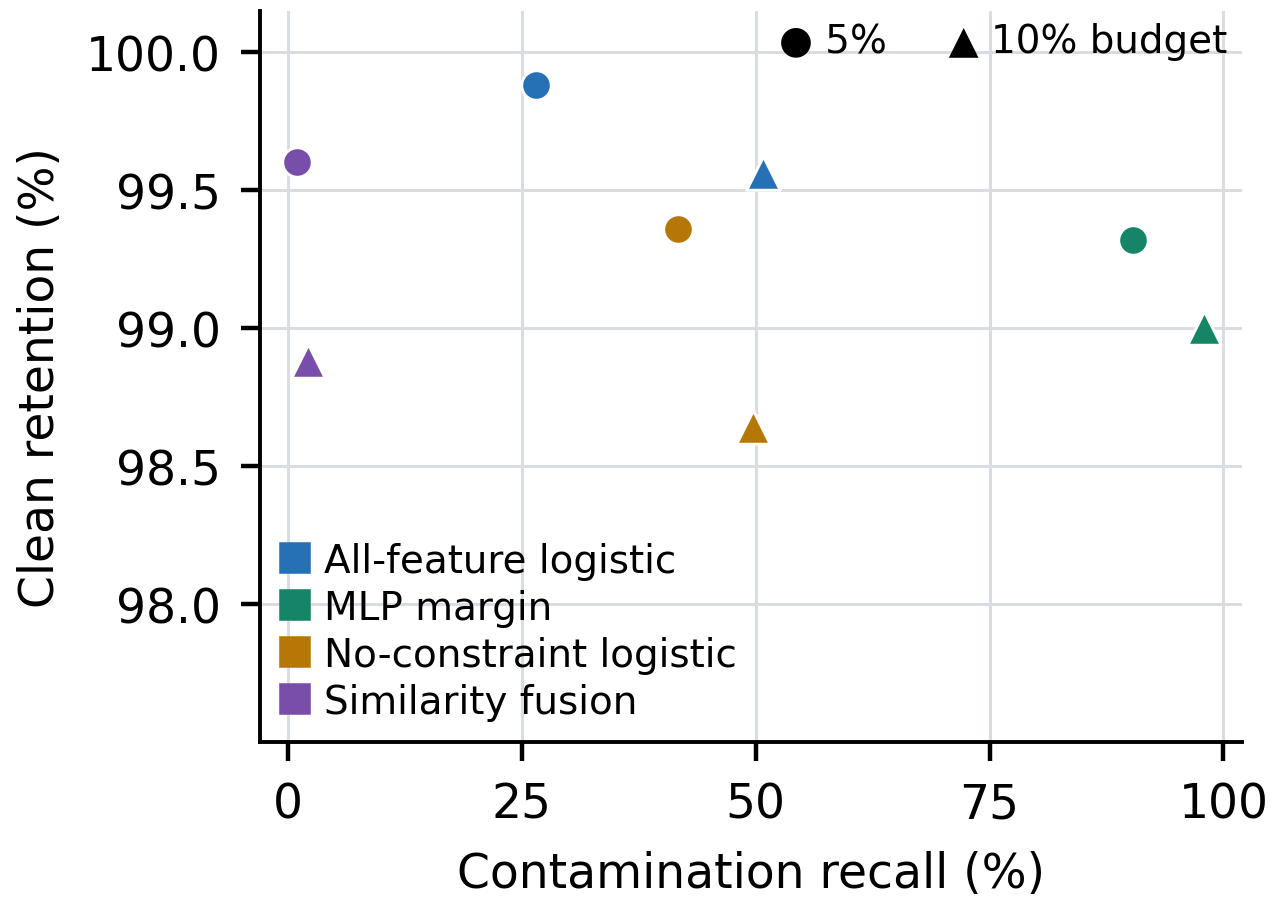
\includegraphics[width=0.745\columnwidth]{fig1_cropped.png}
\caption{Calibrated operating points on the constructed pool at 5\% and 10\% group budgets.}
\label{fig:tradeoff}
\end{figure}

\begin{table}[t]
\caption{Protocol-Valid Raw-Search Locked Tests at the 5\% Budget.}
\label{tab:raw}
\centering
\scriptsize
\setlength{\tabcolsep}{3pt}
\begin{tabular}{@{}llllrrr@{}}
\toprule
Benchmark & Adapter & Pos./clean & Selected & Recall & Clean & AUROC\\
\midrule
MMLU-silver & Full & 68/86 & Logistic & 91.18 & 5.81 & .9518\\
MMLU-human & Full & 82/71 & Logistic & 81.71 & 0.00 & .9894\\
Reasoning Challenge & Light & 17/223 & Logistic & 41.18 & 2.24 & .9053\\
HellaSwag & Light & 22/155 & Word TF--IDF & 63.64 & 0.00 & .9261\\
C-Eval & Light & 129/144 & Logistic & 46.51 & 2.08 & .9273\\
\bottomrule
\end{tabular}
\begin{flushleft}
\tiny Recall and Clean (clean-removal) are source-item-level percentages, not the pair-level rates in~(\ref{eq:pair}). Human excludes one uncertain item. Full includes the frozen embedding model; Light uses lexical and constraint evidence.
\end{flushleft}
\end{table}

\section{Results}
\label{sec:results}
\subsection{Constructed-Pair Sensitivity Study}
On the constructed arithmetic and MCQ pairs in Table~\ref{tab:constructed}, the fixed-configuration MLP-margin rerun reaches 90.34\% CR, 0.68\% pair CDR, and 2.01\% GCDR, and ten grouped re-splits yield $86.67\pm7.50\%$ recall (population SD; 69.99\%--95.03\%). Because configuration and threshold selection inspect calibration outcomes, the MCQ calibration bound of 4.67\% is descriptive rather than a fresh certificate; Section~\ref{sec:raw} reports the final protocol-valid evaluation.

Recall is 92.21\% for arithmetic and 85.43\% for MCQ under the shared threshold, and 68.42\% for MATH under its local threshold; the smaller MATH reservoir also widens its split range. Raising the prespecified group budget from 5\% to 10\% moves the margin threshold from 56.40 to 10.67, raising CR to 97.93\%, pair CDR to 1.00\%, and GCDR to 3.30\%; finite deployment budgets remain fixed before test inspection.

Probability ties from saturated logits produce zero recall in four re-splits; unsquashed margins preserve ordering. The 210 false negatives comprise 98 released rephrasings, 63 other transformations, 30 answer fragments, and 19 exact copies (one GSM8K and 18 MMLU). Of 17 false removals, 14 are GSM-Symbolic re-instantiations~\cite{mirzadeh2024}, two answer-changing GSM-Plus items~\cite{li2024gsmplus}, and one MMLU item from the same audited subjects.

Arithmetic and MCQ margin thresholds transfer poorly to MATH~\cite{huang2025}, removing a retain candidate in 28.95\% and 11.84\% of source groups, while the MATH-calibrated threshold loses 30.99 and 35.34 recall points on arithmetic and MCQ relative to their local thresholds. Local re-estimation corrects the operating point, not evidence absent from the deployed adapter itself.

\subsection{Protocol-Valid Raw Search Audit}
\label{sec:raw}
The raw-search audit uses MMLU search responses and silver annotations released by Li et al.~\cite{li2024}. Joining identifiers, discarding empty responses, and deduplicating uniform resource locators leaves 783 items: 467 clean, 58 input-contaminated, and 258 input-and-label-contaminated. Because archived full pages are unavailable, scoring uses result titles and snippets only, and pages later opened by annotators never enter the frozen features; the source-item split assigns 308/159/162/154 items to training, validation, calibration, and test, and silver labels never enter the feature vector.

Validation compares word and character TF--IDF, frozen Beijing Academy of Artificial Intelligence General Embedding small-en-v1.5 cosine~\cite{xiao2024}, full-evidence logistic regression ($\ell_2$ penalty, $C=1$), and a 16-unit MLP (weight decay $10^{-3}$, L-BFGS) near 5\% empirical clean damage, with concatenated componentwise maxima, top-two means, and overall means of page features for learned scorers; single-feature baselines use maxima. Recall is 53.97\%, 49.21\%, 31.75\%, 79.37\%, and 68.25\%, and AUROC is 0.8980, 0.8848, 0.8328, 0.9431, and 0.8973, so validation selects logistic regression for later MMLU decisions.

Calibration contains 106 retain groups; at a 5\% budget and 95\% confidence ($H=1$), one exceedance is allowed, giving threshold 0.61848 with a one-sided upper bound of 4.397\%. The locked test removes 62/68 silver-contaminated items (91.18\%; group-bootstrap 95\% interval 83.58--97.14\%) and 5/86 silver-clean items (5.81\%; interval 1.25--11.39\%); AUROC is 0.9518. The calibration statement bounds population clean-group risk with 95\% confidence over the random calibration sample, not every finite test split, so the observed 5.81\% does not contradict the 5\% budget.

Human adjudication changes only the evaluation labels; the locked rule removes 67/82 contaminated items (81.71\%; exact 95\% confidence interval 71.63--89.38\%) and 0/71 clean items (one-sided 95\% exact upper bound 4.13\%). Precision is 100\% (confidence interval 94.64--100\%) and AUROC is 0.9894; the uncertain item is excluded. With full-page access, removal is 15/20 contaminated and 0/30 clean (one-sided 95\% exact upper bound 9.50\%). Table~\ref{tab:raw} reports all audits.

Lighter adapters for the Allen Institute for Artificial Intelligence Reasoning Challenge, HellaSwag, and Chinese Evaluation Suite (C-Eval) remove 0--2.24\% of clean items but recall only 41.18--63.64\%. In the web pilot, removal is 90.74\% for answer-bearing records, 81.82\% for question-only records, and 0.00\% for cross-item controls. The frozen English-trained MLP-margin probe removes 0/72 exact-text, 8/72 English, and 2/72 Chinese derivatives (4.63\% overall) after local calibration; the learned scorer has no exact-match override.

\section{Discussion and Validity}
GSM-Plus and GSM-Symbolic show that broad similarity can survive answer changes, while false negatives cluster in paraphrases and short fragments whose decisive content activates few constraints, so the learned combiner and its score scale remain part of the policy. Threshold transfer fails in the same way: arithmetic or MCQ cutoffs delete substantial legitimate MATH material, and English-trained features miss cross-lingual contamination. Threshold transfer violates the matched-distribution assumption: weighted conformal calibration can bound the coverage loss under bounded drift~\cite{barber2023}, whereas SafeDecontam requires a matched reservoir per family and abstains otherwise.

Figure~\ref{fig:tradeoff} compares calibrated operating points; policy evaluation reports CR, CDR, and GCDR as decision metrics, retaining AUROC only as a ranking summary~\cite{bates2021}.

The finite-sample statement bounds population risk at the stated confidence~\cite{clopper1934}, and the 4.13\% one-sided upper bound of the adjudicated audit retains sampling uncertainty. Retrieval must favor sensitivity because misses are unrecoverable~\cite{robertson2009}, whereas deletion uses the frozen adapter, scorer, and threshold~\cite{bates2021}.

Three limitations bound the evidence: MATH-Perturb links use approximate matching~\cite{huang2025}, and constructed-pool feature comparison inspects calibration outcomes. Raw-search calibration uses silver overlap labels~\cite{li2024} and assumes future retain groups follow the calibration distribution; human adjudication improves test labels, but only 51 of 154 items had a full page available to at least one annotator, 103 decisions use snippets, and initial four-class agreement was modest before adjudication, so the human-label result audits the locked decisions rather than certifying human-clean population risk. External audits use lexical and constraint adapters on English and Chinese multiple-choice material; repeated-seed raw-search evaluation, stronger semantic baselines, code and task benchmarks, long documents, obfuscation, timestamped corpora, and additional languages remain untested.

\section{Conclusion}
SafeDecontam converts retrieved benchmark-related evidence into source-level corpus-deletion decisions under a prespecified collateral-damage budget~\cite{bates2021}. On the blinded adjudicated MMLU audit, the locked rule removes 67/82 contaminated and 0/71 clean source items, with a one-sided 95\% exact clean-error upper bound of 4.13\%; lower recall on external families and cross-lingual evidence shows that calibration cannot compensate for retrieval misses or evidence the adapter does not encode. The method is a calibrated deletion policy for retrieved candidates, not an end-to-end guarantee of finding every contaminated record; broader use requires full-page annotation, difficult retain relations, and family-specific calibration data before deployment.

\section*{Acknowledgment}
ChatGPT was used for language editing and LaTeX typesetting. The authors reviewed the manuscript, verified the reported results and citations, and take responsibility for the final text.

\begin{thebibliography}{00}
\bibitem{sainz2023} O. Sainz, J. Campos, I. Garc\'ia-Ferrero, J. Etxaniz, O. L. de Lacalle, and E. Agirre, ``NLP evaluation in trouble: On the need to measure LLM data contamination for each benchmark,'' in \emph{Findings of EMNLP}, 2023, pp. 10776--10787.
\bibitem{deng2024} C. Deng, Y. Zhao, X. Tang, M. Gerstein, and A. Cohan, ``Investigating data contamination in modern benchmarks for large language models,'' in \emph{Proc. NAACL-HLT}, 2024, pp. 8706--8719.
\bibitem{jacovi2023} A. Jacovi, A. Caciularu, O. Goldman, and Y. Goldberg, ``Stop uploading test data in plain text: Practical strategies for mitigating data contamination by evaluation benchmarks,'' in \emph{Proc. EMNLP}, 2023, pp. 5075--5084.
\bibitem{li2024} Y. Li, Y. Guo, F. Guerin, and C. Lin, ``An open-source data contamination report for large language models,'' in \emph{Findings of EMNLP}, 2024, pp. 528--541.
\bibitem{yang2023} S. Yang, W.-L. Chiang, L. Zheng, J. E. Gonzalez, and I. Stoica, ``Rethinking benchmark and contamination for language models with rephrased samples,'' arXiv:2311.04850, 2023.
\bibitem{broder1997} A. Z. Broder, ``On the resemblance and containment of documents,'' in \emph{Proc. Compression and Complexity of Sequences}, 1997, pp. 21--29.
\bibitem{robertson2009} S. Robertson and H. Zaragoza, ``The probabilistic relevance framework: BM25 and beyond,'' \emph{Found. Trends Inf. Retr.}, vol. 3, no. 4, pp. 333--389, 2009.
\bibitem{bates2021} S. Bates, A. Angelopoulos, L. Lei, J. Malik, and M. I. Jordan, ``Distribution-free, risk-controlling prediction sets,'' \emph{J. ACM}, vol. 68, no. 6, Art. 43, 2021.
\bibitem{li2024gsmplus} Q. Li, L. Cui, X. Zhao, L. Kong, and W. Bi, ``GSM-Plus: A comprehensive benchmark for evaluating the robustness of LLMs as mathematical problem solvers,'' in \emph{Proc. ACL}, 2024, pp. 2961--2984.
\bibitem{mirzadeh2024} I. Mirzadeh, K. Alizadeh, H. Shahrokhi, O. Tuzel, S. Bengio, and M. Farajtabar, ``GSM-Symbolic: Understanding the limitations of mathematical reasoning in large language models,'' arXiv:2410.05229, 2024.
\bibitem{huang2025} K. Huang et al., ``MATH-Perturb: Benchmarking LLMs' math reasoning abilities against hard perturbations,'' in \emph{Proc. ICML}, vol. 267, 2025, pp. 25311--25328.
\bibitem{miao2020} S.-Y. Miao, C.-C. Liang, and K.-Y. Su, ``A diverse corpus for evaluating and developing English math word problem solvers,'' in \emph{Proc. ACL}, 2020, pp. 975--984.
\bibitem{clopper1934} C. J. Clopper and E. S. Pearson, ``The use of confidence or fiducial limits illustrated in the case of the binomial,'' \emph{Biometrika}, vol. 26, no. 4, pp. 404--413, 1934.
\bibitem{cobbe2021} K. Cobbe et al., ``Training verifiers to solve math word problems,'' arXiv:2110.14168, 2021.
\bibitem{hendrycks2021mmlu} D. Hendrycks et al., ``Measuring massive multitask language understanding,'' in \emph{Proc. ICLR}, 2021.
\bibitem{hendrycks2021math} D. Hendrycks et al., ``Measuring mathematical problem solving with the MATH dataset,'' in \emph{Proc. NeurIPS Datasets and Benchmarks}, 2021.
\bibitem{patel2021} A. Patel, S. Bhattamishra, and N. Goyal, ``Are NLP models really able to solve simple math word problems?'' in \emph{Proc. NAACL-HLT}, 2021, pp. 2080--2094.
\bibitem{liu2020} J. Liu, L. Cui, H. Liu, D. Huang, Y. Wang, and Y. Zhang, ``LogiQA: A challenge dataset for machine reading comprehension with logical reasoning,'' in \emph{Proc. IJCAI}, 2020, pp. 3622--3628.
\bibitem{lin2022} S. Lin, J. Hilton, and O. Evans, ``TruthfulQA: Measuring how models mimic human falsehoods,'' in \emph{Proc. ACL}, 2022, pp. 3214--3252.
\bibitem{wang2024} W. Wang, S. Jain, P. Kantor, J. Feldman, L. Gallos, and H. Wang, ``MMLU-SR: A benchmark for stress-testing reasoning capability of large language models,'' arXiv:2406.15468, 2024.
\bibitem{xiao2024} S. Xiao, Z. Liu, P. Zhang, N. Muennighoff, D. Lian, and J.-Y. Nie, ``C-Pack: Packed resources for general Chinese embeddings,'' in \emph{Proc. SIGIR}, 2024, pp. 641--649.
\bibitem{barber2023} R. F. Barber, E. J. Cand\`es, A. Ramdas, and R. J. Tibshirani, ``Conformal prediction beyond exchangeability,'' \emph{Ann. Statist.}, vol. 51, no. 2, pp. 816--845, 2023.
\end{thebibliography}

\end{document}
